Für die Durchführung der SMTP Kommunikation wurde das Programm \texttt{telnet} (Version 308) auf einem MacBook Air mit Apple M1-Chip unter macOS 26.5 verwendet.
Die Verbindung zum Server der Universität Münster wurde über das Uni-VPN (Cisco Secure Client) mit dem folgenden Befehl hergestellt:

\codeblock{res/smtp_telnet_command.txt}{Telnet Befehl zum SMTP Verbindungsaufbau}{code:smtp-telnet-command}

Der Server antwortete mit \texttt{220} und bestätigte ESMTP als erweitertes Protokoll.
Anschließend wurden die SMTP Befehle vorbereitet und der Austausch durchgeführt.

\subsection*{Erster Versuch}

Im ersten Versuch wurden alle SMTP Befehle als zusammenhängender Block in Telnet eingefügt.
Der Server akzeptierte die Anfrage und bestätigte die Zustellung mit \texttt{250 ok: Message 406218478 accepted}~\ref{fig:smtp_attempt1}.

\begin{figure}[h]
    \centering
    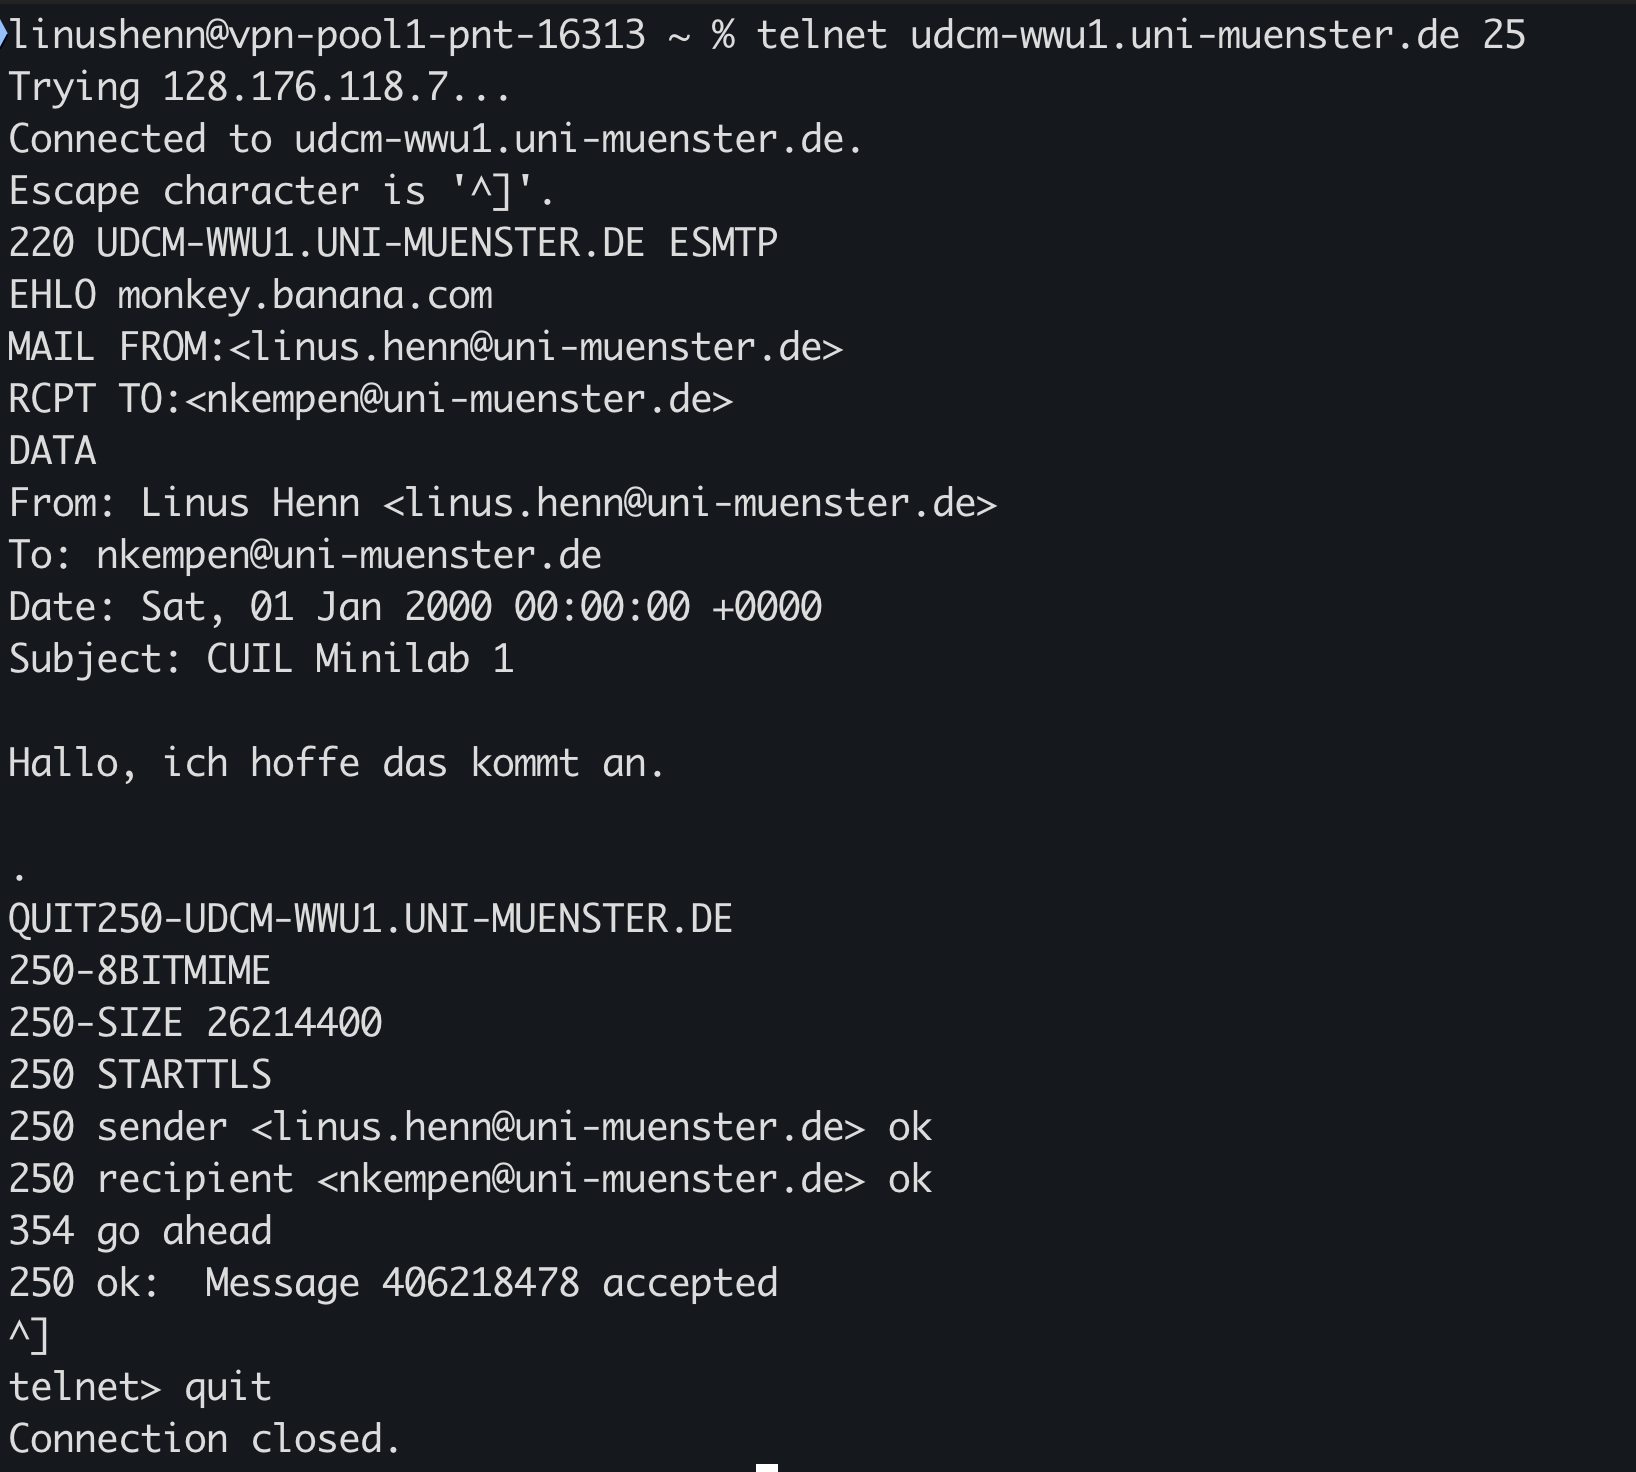
\includegraphics[width=\textwidth]{res/smtp_attempt1.png}
    \caption{Erster SMTP-Versuch: Alle Befehle als Block eingefügt.}\label{fig:smtp_attempt1}
\end{figure}

\FloatBarrier{}

\subsection*{Zweiter Versuch}

Nach erneuter Recherche anhand von RFC 5321 §4.3 wurde festgestellt, dass der Client nach jedem gesendeten Befehl auf die Antwort des Servers warten muss, bevor der nächste Befehl gesendet wird~\cite{rfc5321_smtp}.
Im zweiten Versuch wurden die Befehle daher einzeln geschickt.

\begin{table}[h]
    \centering
    \begin{adjustbox}{max width=\textwidth}
        \begin{tabular}{|c|c|c|}
            \hline
            \textbf{Befehl} & \textbf{Serverantwort} & \textbf{Bedeutung} \\
            \hline
            (\texttt{telnet udcm-wwu1\ldots{} 25}) & \texttt{220 UDCM-WWU1\ldots{} ESMTP} & Server bereit, ESMTP unterstützt \\
            \hline
            \texttt{EHLO monkey.banana.com} & \texttt{250-} Capability-Liste & Client identifiziert sich, Server listet Erweiterungen \\
            \hline
            \texttt{MAIL FROM:<linus.henn@\ldots{}>} & \texttt{250 sender ok} & Absender akzeptiert \\
            \hline
            \texttt{RCPT TO:<nkempen@\ldots{}>} & \texttt{250 recipient ok} & Empfänger akzeptiert \\
            \hline
            \texttt{DATA} & \texttt{354 go ahead} & Server bereit für Nachrichteninhalt \\
            \hline
            (\textit{Header} + \textit{Body}) + \texttt{.} & \texttt{250 ok} & Nachricht zugestellt/akzeptiert \\
            \hline
            \texttt{QUIT} & \texttt{221 UDCM-WWU1\ldots{}} & Verbindung korrekt beendet \\
            \hline
        \end{tabular}
    \end{adjustbox}
    \caption{SMTP Befehle im zweiten Versuch}\label{tab:smtp_dialog}
\end{table}

\FloatBarrier{}

Der Server warb in der EHLO-Response mit den Erweiterungen \texttt{8BITMIME}, \texttt{SIZE 26214400} und \texttt{STARTTLS}.
Der Server antwortete auf \texttt{QUIT} mit \texttt{221} und schloss die Verbindung, was dem korrekten Verbindungsabbau gemäß RFC 5321 §4.1.1.10 entspricht~\cite{rfc5321_smtp}.

\begin{figure}[h]
    \centering
    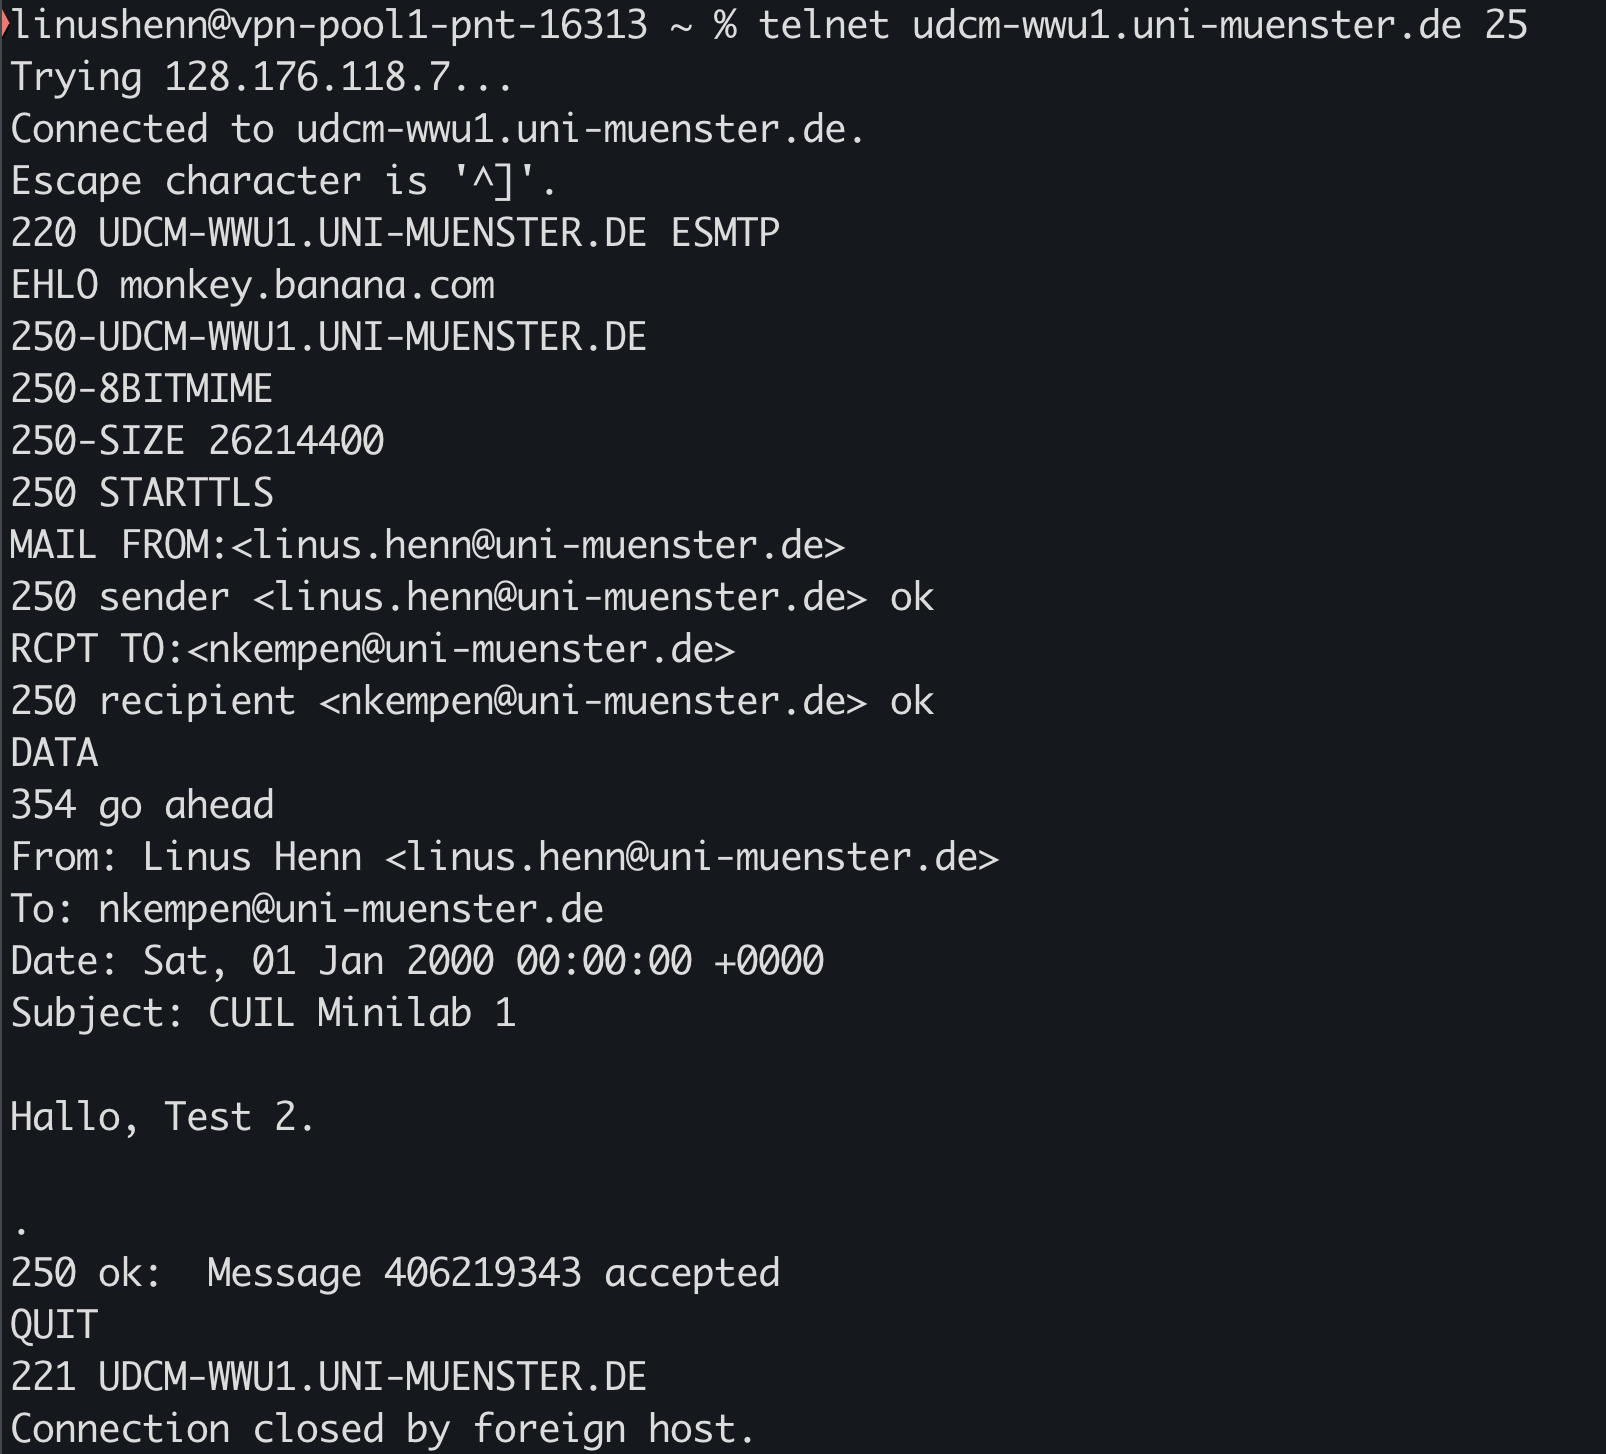
\includegraphics[width=\textwidth]{res/smtp_attempt2.png}
    \caption{Zweiter SMTP Versuch: Korrekte Befehlsfolge}\label{fig:smtp_attempt2}
\end{figure}

\FloatBarrier{}

\subsection*{Auswertung}

Der Erfolg des ersten Versuchs könnte sich durch das Konzept des \textit{SMTP Pipelinings} erklären.
Pipelining wird als das Senden mehrerer SMTP-Befehle, ohne auf die jeweiligen Serverantworten zu Warten bezeichnet~\cite{rfc2920_smtp_pipelining}.

Der Grund könnte zudem in der zugrundeliegenden TCP-Verbindung liegen: TCP garantiert für alle Sendebytes Zuverlässigkeit und richtige Reihenfolge im Empfangspuffer.
Der SMTP Server liest und verarbeitet die Befehle sequenziell aus dem Puffer.

Obwohl Pipelining hier funktionierte, ist dieses Verhalten ohne explizite Serverunterstützung nicht garantiert.
Der Server dieses Versuchs warb nicht mit der Erweiterung \texttt{PIPELINING} nach RFC 2920~\cite{rfc2920_smtp_pipelining}.
Somit wird keine Garantie für korrektes Verhalten bei gepipelinten Befehlen gegeben:
Schlägt ein früher Befehl fehl und befinden sich nachfolgende Befehle aufgrund des Pipelinings bereits im Empfangspuffer, kann es zu undefinierten Zuständen kommen.
Pipelining gibt in diesem Fall Garantie für sicheres Recovery~\cite{rfc2920_smtp_pipelining}.
